\subsection{Oracle Agent}\label{Oracle_Agent}

The oracle agent makes decisions by using the collective experience of all of its units. During each turn, all the units calculate their individual Q-Values based on the outcome of their last state and action. Then, each unit shares this new value with all of its allied units, who copy this Q-Value if they have previously not encountered the corresponding state-action pair. Because it combines all the experience from all its units, we expect the oracle agent to perform better than the cooperative and independent agents.

%The oracle agent makes decisions by using the collective knowledge of all of its units. This agent has the knowledge of the locations of each unit and locations of the enemies which are within range of visible squares of the units. Based on all of this information, the oracle makes a decision for its next move.
 

%Because of combining all the knowledge from all its units, the oracle agent performs better than the cooperative agent. This scenario can be explained with figure-~\ref{fig:coop_vs_oracle}. %Here we consider a $3*3$ board where the visible square is $1$. Now if black circled units are controlled by the cooperative agent then unit-1 will have no knowledge of unit-2. So both will try to attack the enemy unit-A. Which ever unit kills enemy unit-A first will die by the second attacking ally unit. On the other hand if the black circled units are controlled by oracle agent then the agent will choose one unit from unit-1 and unit-2 based on their Q-values to attack unit-A
%Here we consider a $3$ by $3$ board where the visible range is $1$. Now if black circled units are controlled by the cooperative agent then unit-1 will have no knowledge of unit-2, so both will try to attack the enemy unit-A. Whichever unit kills enemy unit-A first will die by the second attacking the ally unit. On the other hand if the black circled units are controlled by oracle agent then the agent will choose either unit-1 or unit-2 based on their Q-values to attack unit-A



%\begin{figure}[htb]

%\begin{minipage}[b]{1.0\linewidth}
 % \centering
 % \centerline{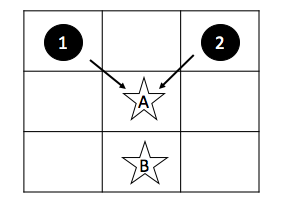
\includegraphics[width= 3.5 cm]{coop_vs_oracle}}
%  \vspace{2.0cm}
  
%\end{minipage}
%\caption{Comparing movements of oracle agent with cooperative agent}
%\label{fig:coop_vs_oracle}
%
%\end{figure}
